\procTitle{Распределение скорости смещения обломочного чехла в~аккумулятивных частях коллювиальных конусов в~горах Дел-Урэкчэн (Северное Приохотье) по~лихенометрическим данным}
\procTitleNewLine{Распределение скорости смещения обломочного чехла в~аккумулятивных частях коллювиальных конусов\\в~горах Дел-Урэкчэн (Северное Приохотье)\\по~лихенометрическим данным}
\procAuthor{Колегов~П.\,П., Кондратьев~М.\,Н.}
\procEmail{kolegovpp@gmail.com, mkondratyev85@gmail.com}
\procOrganization{СВКНИИ ДВО РАН} \procCity{Магадан}

\makeProcTitleNewLine
\index{k@Колегов~П.\,П.}
\index{k@Кондратьев~М.\,Н.}

Рассматривая процессы склонового морфолитогенеза на территории Северного Приохотья,
можно выделить следующие типы: обваливание, осыпание, десерпция, плоскостной смыв, солифлюкция.
Их изучением на Северо-Востоке Азии занимались разные исследователи с переменным успехом.
Стоит отметить работы Т.\,И.\,Каплиной, посвящённые криогенным образованиям
и солифлюкции в частности [4]; Э.\,Э.\,Титова описавшего типы коллювиальных образований
и их взаимосвязь с криолитозоной [9, 10]; В.\,Л.\,Суходровского, разработавшего классификацию рельефообразующих процессов криолитозоны [8].

Начиная с 2000-х гг. стали применять новые количественные и качественные методы (лихенометрия, анализ космических снимков высокого разрешения) при изучении динамики склоновых процессов,
что возобновило интерес к исследованиям в данной области. Здесь можно выделить работы В.\,Н.\,Смирнова и А.\,А.\,Галанина [1--3].

Нами проведены исследования по динамике и цикличности процессов, формирующих коллювиальные конусы выноса на территории Северного Приохотья (центральная часть гор Дел-Урэкчэн), в ходе которых получены количественные данные по скорости смещения обломочного чехла (0,2--2,0\,м/год), динамического возраста (300--500\,лет) и выявлены геопространственные закономерности в размещении данных форм [5--7].

Целью данных исследований было выявление закономерности в распределении скорости смещения обломочного чехла в разных частях аккумулятивной зоны.

Участок исследования расположен в правом борту р.~Нельканджа (басс. р.~Армань) близ слияния с р.~Нанкала (60\dg16’48”\,с.\,ш., 150\dg56’42”\,в.\,д.). Рельеф участка среднегорный, абсолютные отметки высот водоразделов составляют 850--900\,м, долины~--- 530--560\,м (рис.\,1, слева). Ширина долины составляет 1500~м, поймы до 200~м. Форма долины U-образная. Вдоль бортов долин сохранились реликты моренных накоплений последних оледенений. Склоны крутые (25--35\dg), покрытые маломощным обломочным чехлом, коренные выходы на них редки.

Для описание рельефа использовалась новая цифровая модель~--- ArcticDEM [11], которая имеет разрешение 2 м/пиксель.

Изученный нами коллювиальный конус имеет следующие морфометрические характеристики, м: длина~---  450, ширина транзитной части~---  15--25, аккумулятивной~--- 115; угол наклона транзитной части~--- 19--26\dg, аккумулятивной~--- 12--18\dg. Превышение области питания над дистальной частью (высота морфоскульптуры)~--- 200~м. Правая часть аккумулятивной зоны (если ориентироваться вниз по склону) имеет превышение в 5~м относительно левой (анализ цифровой модели).

Обломочный чехол сложен крупнощебнистым и мелкоглыбовым материалом в аккумулятивной зоне и мелко-, среднещебнистыми отложениями с дресвяным заполнителем в~транзитной. Петрографический состав обломков представлен риолитами.

%TODO: масштабная линейка на космоснике
\begin{figure}[H]
  \centering
  \includegraphics[width=1\textwidth, page=1]{authors/Kolegov-fig.pdf}
  \caption{Цифровая модель рельефа [11] участка Нельканджа (слева) и космоснимок фронтальной части конуса (справа). Условные обозначения: 1~--- лихеометрическая площадка и её номер; 2~--- направления транзита обломков и их скорость, м/год; на левом рисунке~--- горизонтали проведены через 50\,м, на правом~--- толстые через 10\,м, тонкие через 1\,м. На левой врезке~--- географическое положение участка исследования}
  \label{fig:kolegov-fig}
\end{figure}

В основании конуса, а также в транзитной части были заложены 4 площадки (см. рис.\,1, справа). Методика работ описана нами ранее в [5, 6], но имеются небольшие различия, а~именно были выбраны следующие параметры лихенометрической съёмки:  размер площадки~--- 20\,$\times$\,20\,м; лишайник-индикатор~--- \textit{Rhizocarpon}~sp.; количество замеров на площадке~--- 25 случайно выбранных обломков горной породы; метод измерения~--- самый крупный таллом на обломке; точность измерения~--- 1~мм.

Данное количество замеров на одной площадке обусловлено проведёнными нами статистическими исследованиями методом Монте-Карло базы данных лихенометрической съёмки (70 площадок по 100 замеров) за 2010--2017 гг. Из генеральной совокупности измерений по каждой площадке делались 100 выборок по 25 замеров (рис. 2,\textit{а}). Средняя величина ошибки в определении возраста по сравнению с измерением 100 талломов составляет от 8 до 18\,\%, для интервала 200--500\,лет (рис. 2,\textit{б,в}).  Полученные показатели ошибки признаны допустимыми для многопрофильной съёмки в аккумулятивных частях конусов выноса.



Диаметр таллома пересчитан в возраст по уравнению [6]:

$$t = 1000\cdot ln{\left(-\frac{1}{d-230}\right)}+5438,02,$$

где $t$~--- возраст таллома; $d$~--- максимальный диаметр лишайника, рассчитанный по убывающему логарифмическому тренду выборки из 25 измерений.

Основные показатели лихенометрического анализа приведены в таблице. Отметим, что полученные значения характерны для поверхностного слоя мощностью не~более 20~см.

\begin{figure}[H]
  \begin{center}
    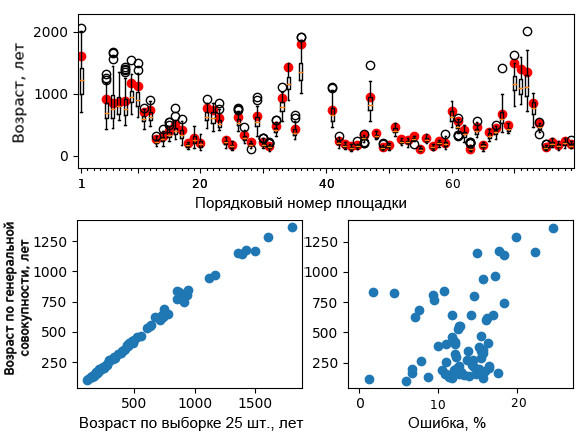
\includegraphics[width=0.8\textwidth]{authors/kolegov-fig2.jpg}
  \end{center}
  \caption{График распределения выборок (\textit{а}). Красными точками показаны истинные значения,
полученные по 100 замерам, черные боксы и кружки~--- выборки из 25 шт. Графики ошибок: \textit{б}~--- график зависимости истинных значений от выборки в 25 ед. \textit{в}~--- погрешность измерений получаемая при замере 25 шт. талломов}
  \label{fig:kolegov}
\end{figure}


\begin{changemargin}{-2cm}{-2cm}

\begin{center}
\begin{minipage}[c]{1.2\textwidth}
 \begin{table}[H]
 \begin{center}
 \caption*{\bfseries Индексы генетического разнообразия и тестов на нейтральность в исследованных популяциях}
 
 \label{tab:litvinov1}
 \medskip\small
 \begin{tabularx}{1.0\linewidth}{l c c r c r c c }
 \toprule
 %Русские юго-запад &
 \parbox[c][8em][c]{0.06\textwidth}{ \centering Про\-филь} &
 \parbox[c][8em][c]{0.10\textwidth}{ \centering Угол наклона поверхности осыпи, °} &
 \parbox[c][8em][c]{0.10\textwidth}{ \centering Длина поверхности осыпи, м} &
 \parbox[c][8em][c]{0.10\textwidth}{ \centering Площадь поверхности осыпи, м$^2$} &
 \parbox[c][8em][c]{0.08\textwidth}{ \centering Скорость транзита облом. чехла, м/год} &
 \parbox[c][8em][c]{0.12\textwidth}{ \centering Энерге\-тический потенциал, кДж} &
 \parbox[c][8em][c]{0.10\textwidth}{ \centering Удельный энергет. потенциал ($E_{\textup{уд.}}$), кДж/м$^2$} &
 \parbox[c][8em][c]{0.10\textwidth}{ \centering Удельный энергет. потенциал ($A_{\textup{уд.}}$), кДж/м$^2$}\\

 \midrule

 1 &
 30 &
 143 &
 8\,071 \hspace*{0.3cm}&
 0,67 &
 2,94$\cdot$10$^6$ &
 364,56 &
 1,70 \\
 5 &
 20 &
 194 &
 12\,620 \hspace*{0.3cm}&
 0,38 &
 4,64·10$^6$ &
 368,02 &
 0,71 \\
 8 &
 23 &
 304 &
 22\,740 \hspace*{0.3cm}&
 1,09 &
 14,62·10$^6$ &
 643,30 &
 2,30 \\
 10 &
 23 &
 108 &
 4\,014 \hspace*{0.3cm}&
 0,20 &
 0,92·10$^6$ &
 229,75 &
 0,42 \\
 11 &
 26 &
 145 &
 5\,247 \hspace*{0.3cm}&
 0,33 &
 1,77·10$^6$ &
 337,67 &
 0,76 \\
 12 &
 28 &
 118 &
 5\,000 \hspace*{0.3cm}&
 0,79 &
 1,45·10$^6$ &
 289,85 &
 1,92 \\


 \bottomrule
 \end{tabularx}
 \end{center}

 \end{table}
\end{minipage}
\end{center}
\end{changemargin}

\bigskip


\clearpage

Анализ полученных данных позволяет сделать следующие выводы:

\begin{enumerate}[noitemsep]\vspace{-8pt}
  \item допустимо при лихенометрической съёмке производить 25 замеров талломов, при этом погрешность относительно обычной методики (100~замеров) составит 8--15\,\%;
  \item скорость транспортировки обломков в различных частях аккумулятивной зоны варьирует от~0,17 до~0,53~м/год, при среднем значении 0,34~м/год;
  \item динамический возраст поверхности аккумулятивной зоны варьирует от 268 до 502 лет в разных её частях.
\end{enumerate}



\begin{thebibliography}{99}
%1
\bibitem{}\BibAuthor{Галанин\,А.\,А.} Лихенометрия: современное состояние и направление развития
метода (аналитический обзор).~--- Магадан~: СВКНИИ ДВО РАН, 2002.~--- 74~с.
%2
\bibitem{}\BibAuthor{Галанин\,А.\,А.} Каменные глетчеры Северо-Востока России: строение, генезис,
возраст, географический анализ~: дис. $\dots$ д-ра наук.~--- Владивосток, 2009.~--- 303~с.
%3
\bibitem{}\BibAuthor{Галанин\,А.\,А., Смирнов\,В.\,Н.} Динамика гравитационных склоновых процессов в горах Северного Приохотья в позднем голоцене и лихенометрическая методика их моделирования и прогноза // Геоморфология.~--- 2004.~--- №~3.~--- С.~67--75.
%4
\bibitem{}\BibAuthor{Каплина\,Т.\,И.} Криогенные склоновые процессы.~--- М.~: Наука, 1965.~--- 296~с.
%5
\bibitem{}\BibAuthor{Колегов\,П.\,П.} Динамика коллювиальных процессов в хребте Дел-Урэкчэн (Северное Приохотье) на основе лихенометрических данных // Вестник СВНЦ ДВО РАН.~--- 2016.~--- №~2.~--- С.~10--18.
%6
\bibitem{}\BibAuthor{Колегов\,П.\,П.} Динамика осыпей и каменных глетчеров Ольского плато (Северное Приохотье) на основании лихенометрического и фотометрического гранулометрического анализов // Там же.~--- 2019.~--- №~3.~--- С.~54–62.~--- DOI: 10.34078/1814-0998-2019-3-54-62.
%7
\bibitem{}\BibAuthor{Колегов\,П.\,П.} Геопространственный анализ коллювиальных конусов выноса центральной части гор Дел-Урэкчэн (Северное Приохотье) // Форум <<Наука Северо-Востока России: фундаментальные и прикладные исследования в Северной Пацифике и Арктике>>. Магадан, 5--6 марта 2020~г. / отв. ред. Н.\,А.\,Горячев.~--- Магадан~: СВКНИИ ДВО РАН, 2020.~--- С.~41--44.
%8
\bibitem{}\BibAuthor{Суходровский\,В.\,Л.} Экзогенное рельефообразование в криолитозоне.~--- М.~:
Наука, 1979.~--- 280~с.
%9
\bibitem{}\BibAuthor{Титов\,Э.\,Э.} Скорости перемещения обломочного материала на склонах гор
Северо-Востока СССР // Вестник МГУ. География.~--- 1970.~--- №~4.~--- С.~95--98.
%10
\bibitem{}\BibAuthor{Титов\,Э.\,Э.} Строение и развитие склонов гор Северо-Востока СССР~: автореф.
дис. $\dots$ канд. геогр. наук.~--- Мoсква, 1971.~--- 35~с.

\bibitem{}ArcticDEM~--- Polar Geospatial Center // University of Minnesota.~--- 2018.~--- URL: https://www.pgc.umn.edu/\-data/arcticdem (ref. date: 20.02.2020).

\end{thebibliography}
\thispagestyle{empty}
